\documentclass{article} % For LaTeX2e
\usepackage{nips15submit_e,times}
\usepackage{hyperref}
\usepackage{url}
\usepackage[
    backend=biber,
    style=ieee,
    sorting=ynt
]{biblatex}
\usepackage{amsmath}
\usepackage{amsfonts}
\usepackage{bbm}
\usepackage{graphicx}
\usepackage{float}
\usepackage{tikz}
\usepackage{algpseudocode}
\usepackage{algorithm}

\addbibresource{ref.bib}

\title{Reinforcement Learning Methods for Training Simulated Autonomous Robots Inside Habitat-Lab}

\author{
Riley Francis \\
BS Computer Science, BA Mathematics \\
School of Computing \\
University of Connecticut \\
riley.francis@uconn.edu
\thanks{I want to give special thanks to my mentor, Dr. Jonathan Shihao Ji for his continuous help and support throughout this project, as well as to my collaborators Marcus Maravilla, Grace McPadden, Abeshan Javed, and Martha Condori for their assistance.}
}

\newcommand{\fix}{\marginpar{FIX}}
\newcommand{\new}{\marginpar{NEW}}

\usepackage{listings}
\usepackage{xcolor}

% Define YAML syntax highlighting
\lstdefinelanguage{YAML}{
  keywords={true,false,null,y,n},
  keywordstyle=\color{blue}\bfseries,
  basicstyle=\ttfamily\footnotesize,
  comment=[l]{\#},
  commentstyle=\color{gray},
  stringstyle=\color{teal},
  % moredelim=[l][\color{orange}]{:},   % color colons
  morestring=[b]",
  literate=
   *{0}{{{\color{purple}0}}}{1}
    {1}{{{\color{purple}1}}}{1}
    {2}{{{\color{purple}2}}}{1}
    {3}{{{\color{purple}3}}}{1}
    {4}{{{\color{purple}4}}}{1}
    {5}{{{\color{purple}5}}}{1}
    {6}{{{\color{purple}6}}}{1}
    {7}{{{\color{purple}7}}}{1}
    {8}{{{\color{purple}8}}}{1}
    {9}{{{\color{purple}9}}}{1}
}

% Set your style using the YAML language
\lstdefinestyle{yamlstyle}{
  language=YAML,
  backgroundcolor=\color{gray!10},
  frame=single,
  rulecolor=\color{gray!50},
  breaklines=true,
  tabsize=2,
  showstringspaces=false
}




\nipsfinalcopy % Uncomment for camera-ready version

\begin{document}

\maketitle
\begin{abstract}
Training autonomous navigation policies for real-world robots is difficult due to safety concerns, hardware wear, and the inconsistencies of real-world environments. Robust simulation provides a practical alternative, allowing robots to be trained efficiently and reproducibly at scale. In this work, we use Meta AI’s Habitat-Lab framework—together with the \texttt{kin2dyn} extension for articulated legged robots to train a navigation policy for the Boston Dynamics Spot robot in photorealistic indoor environments. Using Proximal Policy Optimization (PPO) and distributed rollout collection, the agent learns to navigate toward goal locations using only depth observations and goal direction information. We evaluate performance across scenes from the HM3D dataset and analyze training behavior through success metrics, collision trends, and qualitative rollout visualizations. The results demonstrate that Spot can acquire robust point-to-point navigation behaviors within Habitat’s simulation environment. This work has significant potential for transfer to real hardware and outline applications where simulation-trained legged navigation policies could be deployed.
\end{abstract}

\section{Introduction}
Developing autonomous navigation behaviors for real-world robots is a central goal in robotics and embodied AI. Legged robots such as the Boston Dynamics Spot (see \textit{Figure \ref{fig:SpotFig}}) are particularly appealing for navigation tasks because they can handle uneven terrain, steps, and cluttered environments more effectively than wheeled platforms. However, training these systems directly on physical hardware and under real-world conditions is challenging. Reinforcement learning (RL) algorithms typically require large amounts of trial-and-error experience, which is time consuming, risky for expensive hardware, and difficult or impossible to reproduce across different testing conditions. For these reasons, high-fidelity and efficient robotics simulation has become an essential tool for training and evaluating robot learning methods. 

Meta AI’s Habitat platform has emerged as a widely used environment for simulation-based robotics research. Habitat-Sim provides fast, photo-realistic rendering of large indoor spaces, while Habitat-Lab adds a flexible API for defining tasks, sensors, datasets, and RL pipelines. These tools allow us to run thousands of simulation steps per second, making large-scale RL training in any reasonable timescale feasible.

While Habitat has been used extensively for navigation tasks, most applications involve simpler agents such as differential-drive robots or mobile manipulators. Legged robots, which have more complex kinematics and require more advanced control pipelines, have received less attention. The \texttt{kin2dyn} branch of Habitat-Lab, developed by Joanne et al., addresses this issue by introducing URDF-based quadruped models, improved contact and articulation handling, and a unified interface for converting high-level velocity commands into physically simulated locomotion. This makes it possible to train the Spot robot in realistic indoor environments with detailed sensor feedback and accurate physical behaviors.

In this project, we use reinforcement learning—specifically the Proximal Policy Optimization (PPO) algorithm—to train a navigation policy for Spot inside Habitat-Lab using the \texttt{kin2dyn} framework. We focus on the PointNav task, where the robot must reach a target location using depth observations and goal direction information. Our work explores how Habitat’s simulation capabilities, combined with reward shaping and continuous control, affect the robot’s ability to learn reliable navigation behaviors.

By integrating Habitat-Lab’s RL infrastructure with the detailed quadruped model provided by \texttt{kin2dyn}, we show that it is practical to train legged navigation policies entirely in simulation. This approach provides a controlled and scalable way to study autonomous locomotion and lays the foundation for future real-world transfer to physical quadrupedal robots.

\begin{figure}
    \centering
    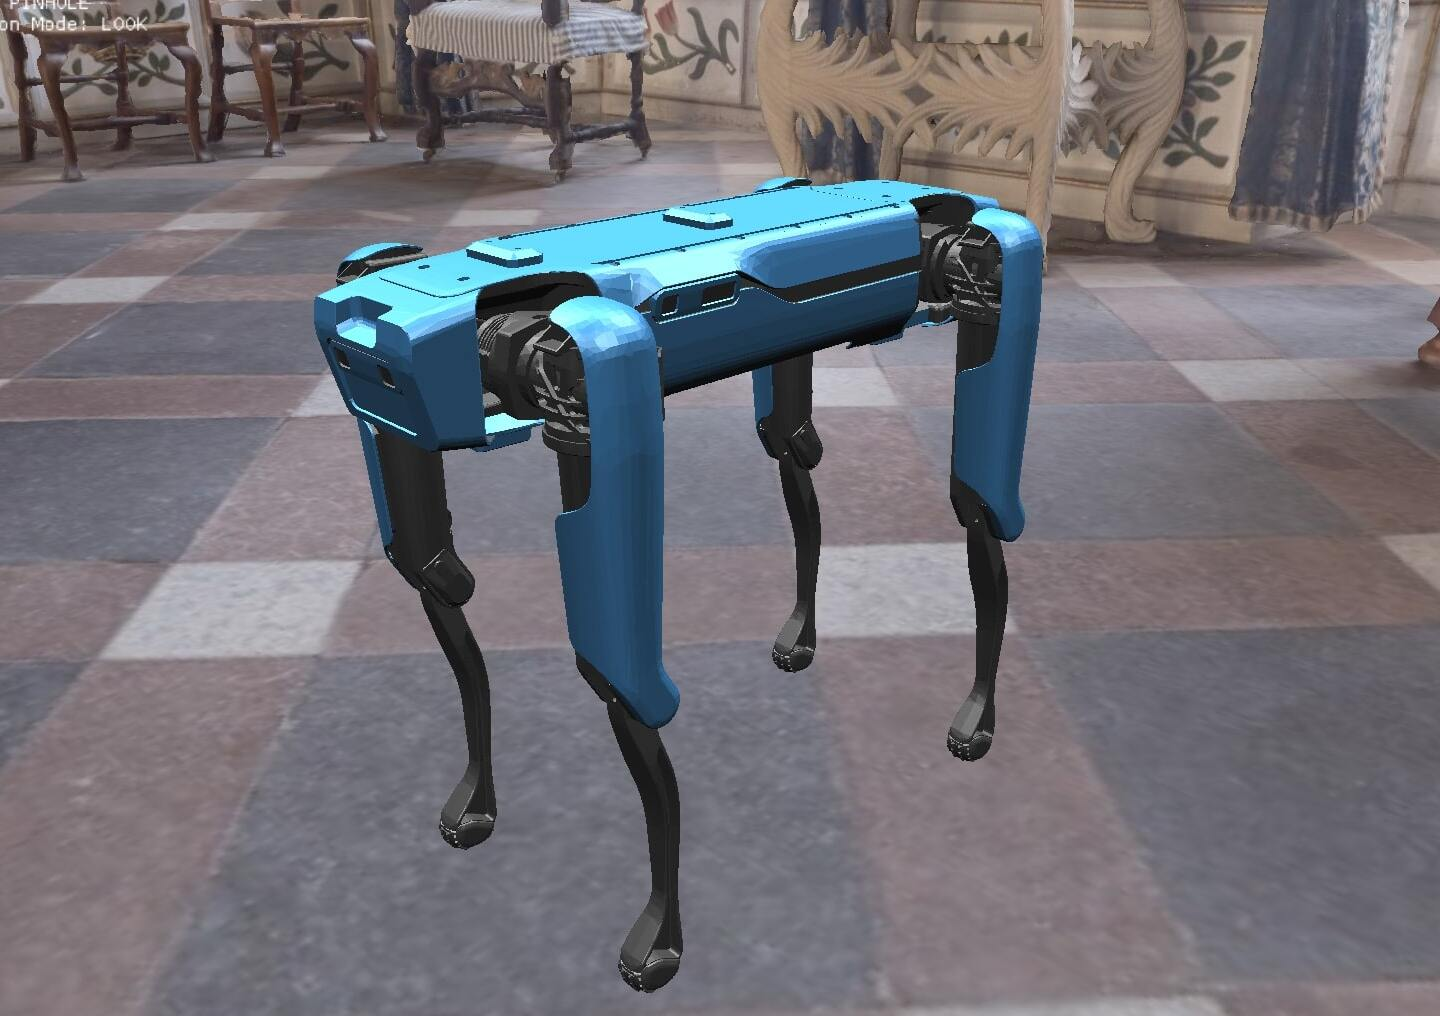
\includegraphics[width=0.45\linewidth]{Images/Spot_Habitat.jpg}
    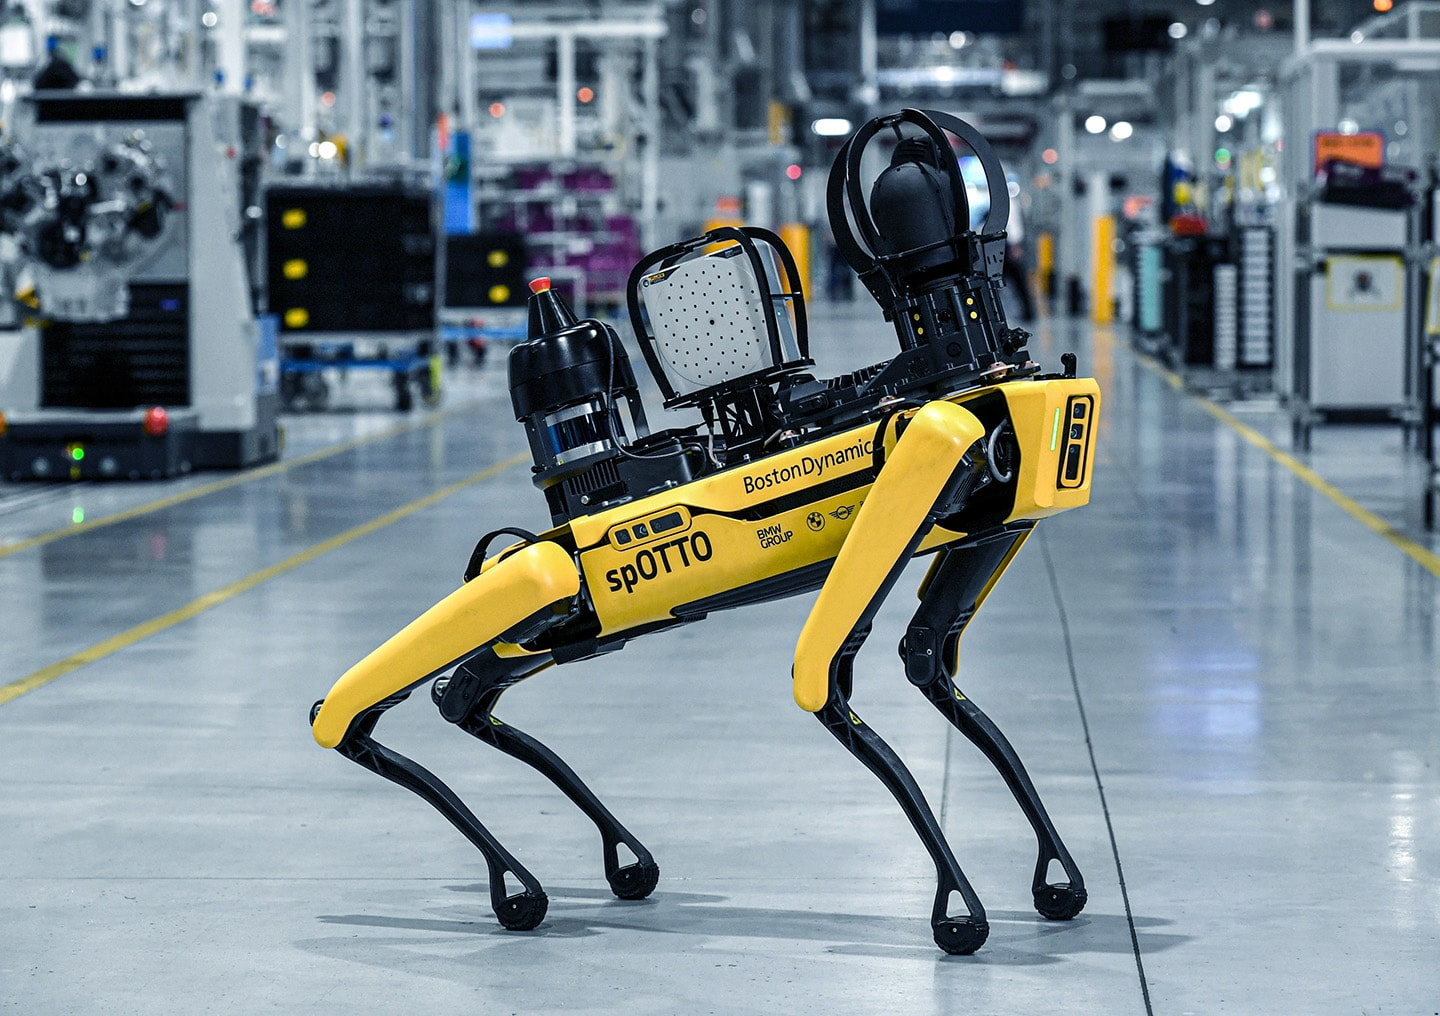
\includegraphics[width=0.45\linewidth]{Images/spot.jpg}
    \caption{This figure shows the Boston Dynamics Spot robot. The left image is the URDF file that we use in our experiments, situated in the \textit{Skokloster's Castle} test scene, and the right image is a real-life Spot robot.}
    \label{fig:SpotFig}
\end{figure}

\section{Related Work}
This section provides an overview of prior research and tools that form the foundation of our approach to training autonomous navigation behaviors in simulation. We first discuss key developments in embodied AI navigation, including common benchmark tasks and methodological trends that influence how agents perceive and act within complex indoor environments. We then examine the high-performance simulation platforms that enable large-scale training, with a focus on Habitat-Sim and Habitat-Lab, which together provide the rendering, physics, and task APIs used in modern embodied learning research. Finally, we highlight recent advances in legged robot simulation—particularly the \texttt{kin2dyn} extension of Habitat-Lab—which introduce articulated quadruped models, improved contact handling, and interfaces suitable for learning realistic locomotion policies. Together, these lines of work contextualize our design choices and motivate the use of Habitat-Lab and reinforcement learning methods for training navigation policies for the Boston Dynamics Spot robot.

\subsection{Embodied AI and Navigation Benchmarks}
Embodied AI focuses on training robotic agents that perceive and act within realistic 3D environments, making navigation one of its central research tasks. A common family of benchmarks in this area includes PointNav \cite{zhao2021surprising}, ObjectNav \cite{batra2020objectnav}, and related indoor navigation challenges. In the PointNav task, the agent receives the relative direction and distance to a target point and must reach it efficiently using onboard devices such as depth sensors, RGB or greyscale cameras, or LiDAR. ObjectNav extends this by requiring the agent to locate a specific object category (e.g., “chair”), thus adding semantic understanding to the problem.

These benchmarks have become standard for evaluating navigation policies because they require agents to combine perception, mapping, planning, and control in realistic 3D spaces. The Habitat platform has played a major role in standardizing these tasks by providing large-scale datasets, consistent success metrics, and high-performance simulation tools. Our work builds directly on the PointNav benchmark, adapting it for quadrupedal control using the Boston Dynamics Spot model within Habitat-Lab’s \texttt{kin2dyn} framework.

\subsection{Habitat-Sim}
Habitat-Sim \cite{habitat19iccv,szot2021habitat,puig2023habitat3} is a high-performance 3D simulator designed to support research in embodied AI, visual navigation, and mobile robotics. Its rendering engine is optimized for large-scale photo-realistic environments, supporting physics-based simulation. Unlike traditional robotics simulators that prioritize physics fidelity, Habitat-Sim focuses on scalable perception-driven tasks, enabling thousands of parallelized simulation steps per second. This emphasis on speed and large-scale training has made Habitat-Sim a core platform for research on navigation policies, embodied exploration, and embodied foundation models. Many state-of-the-art indoor navigation benchmarks, including PointNav\cite{partsey2022mapping}, ObjectNav\cite{batra2020objectnav}, and the HM3D\cite{chang2017matterport3d,ramakrishnan2021habitat} dataset, are built on top of Habitat-Sim’s scene-graph and sensor framework.

\subsection{Habitat-Lab}
Habitat-Lab \cite{habitat19iccv,szot2021habitat,puig2023habitat3} is a modular research library that builds upon Habitat-Sim to provide task definitions, reinforcement learning pipelines, dataset interfaces, and distributed training infrastructure. Habitat-Lab formalizes embodied tasks (e.g., PointNav, ObjectNav, Rearrangement) through standardized interfaces for observations, actions, rewards, and success metrics. Its integration with Habitat-Baselines offers turnkey implementations of common RL algorithms such as PPO, DDPPO, and SAC, along with utilities for multi-GPU rollout collection and evaluation. 

Habitat-Lab has been used extensively for benchmarking autonomous mobile robots in simulated indoor environments, making it a central framework for embodied AI research. For quadrupedal locomotion tasks, Habitat-Lab provides a clean abstraction layer that allows high-level navigation policies to be learned independently of low-level physics, making it well-suited for experiments with robots such as Spot that rely on velocity or kinematic control. Our work builds directly on Habitat-Lab’s PointNav infrastructure, adapting it for high-frequency control of a kinematic quadruped model.

\subsubsection{Habitat-Lab's kyn2dyn Legged Navigation Branch }

The \texttt{kin2dyn}\footnote{For more information on this branch of Habitat-Lab, please refer to the paper published by Truong et al. \cite{truong2022kin2dyn} and their GitHub repository found at \url{https://github.com/joannetruong/habitat-lab/tree/kin2dyn}} branch of Habitat-Lab , introduced by Truong et al. \cite{truong2022kin2dyn}, extends the original framework of Habitat-Lab by supporting legged robots and hybrid kinematic–dynamic control pipelines. Traditional Habitat-Lab agents, such as LoCoBot or Fetch, rely on simple differential-drive or arm kinematics. In contrast, \texttt{kin2dyn} incorporates articulated URDF-based models of quadrupeds, improved contact handling, and a unified control interface that maps high-level velocity commands into dynamically simulated locomotion using NVIDIA PhysX. This modification enables legged robots such as Boston Dynamics Spot or Unitree's A1 robotic dog to be trained in complex navigation tasks within photo-realistic indoor environments. The branch also introduces improved robot articulation, terrain-aware foot placement, and an API for integrating proprioceptive sensors. Recent work using \texttt{kin2dyn} has demonstrated the feasibility of training navigation policies entirely in simulation and deploying them onto real hardware with minimal fine-tuning. In this project, we rely on the \texttt{kin2dyn} branch to simulate Spot’s 17-DOF morphology, generate realistic depth observations, and execute continuous velocity commands suitable for PPO-based locomotion learning.

\section{Methodology}
In this section, we outline the approach used to train a point-to-point navigation policy for the Boston Dynamics Spot robot inside the Habitat-Lab simulation environment. We begin by outlining the reinforcement learning methods of the task, including the sensor observations, continuous control actions, and reward components that shape the agent’s behavior. We then present the Proximal Policy Optimization (PPO) algorithm and its distributed extension (DDPPO), which together enable scalable training across many simulated environments. Finally, we detail the simulation tools, robot model, and dataset configuration provided by Habitat-Lab and the \texttt{kin2dyn} framework that make it possible to train realistic legged locomotion policies entirely in simulation.

\subsection{Reinforcement Learning (RL)}
Reinforcement Learning (RL) is a machine learning method in which an autonomous agent learns to make sequential decisions by interacting with an environment and receiving feedback in the form of rewards. Formally, this process is modeled as a Markov Decision Process (MDP) defined by the tuple $(\mathcal{S},\mathcal{A},P,R,\gamma)$, where $\mathcal{S}$ is the state space, $\mathcal{A}$ the action space, $P(s' \mid s, a)$ the transition dynamics, $R(s,a)$ a scalar reward function, and $\gamma$ a discount factor that weights long-term versus immediate outcomes. The objective is to learn a policy $\pi(a \mid s)$ that maximizes the expected discounted return
\begin{equation}
J(\pi) = \mathbb{E}\Big[\sum_{t=0}^\infty \gamma^t R(s_t,a_t)\Big].
\end{equation}
A high-level view of this interaction loop, showing how observations, actions, rewards, and policy updates are connected, is illustrated in Figure~\ref{fig:rl_diagram}.

In the context of our navigation task, the agent corresponds to the Boston Dynamics Spot robot simulated inside Habitat-Lab, and the environment consists of 3D indoor scenes drawn from the HM3D dataset (see \textit{Section \ref{sec:scene_data}}). At each timestep, Spot receives sensory observations---such as depth images and goal vectors---and outputs continuous velocity commands that determine its motion. Because the dynamics of legged robots are highly nonlinear and the environment contains rather complex geometry, obtaining an analytical model of the transition distribution $P$ is infeasible. This motivates the use of model-free RL methods, which learn directly from experience without requiring an explicit model of the environment.

Model-free RL algorithms can be broadly classified into value-based and policy-based methods. Value-based approaches (e.g., Q-learning) become difficult to scale to high-dimensional continuous action spaces, such as the three-dimensional velocity commands used by Spot. Consequently, we adopt a policy-gradient approach in which the policy is parameterized by a deep neural network and optimized directly through stochastic gradient ascent on the expected return. This formulation is well-suited to robotics because it allows smooth, continuous control and naturally incorporates noisy, partial observations.

Habitat-Lab’s distributed RL backend enables us to train such policies efficiently by running multiple parallel simulators to produce trajectories for gradient updates. Each rollout consists of sequences of states, actions, rewards, and value predictions that are aggregated to update the policy. Through repeated interaction and optimization, the agent gradually discovers behaviors that balance progress toward the goal, collision avoidance, and stable locomotion.

\begin{figure}
    \centering
    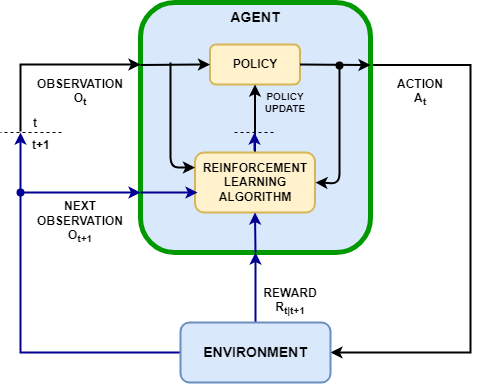
\includegraphics[width=0.75\linewidth]{Images/agent_diagram.png}
    \caption{This figure \cite{MathWorks} shows the reinforcement learning loop used in Habitat-Lab. The agent’s policy generates continuous velocity actions from depth-based observations, interacts with the simulated environment, and receives rewards and next observations. The PPO algorithm processes these transitions to update the policy parameters, improving navigation performance over time.}
    \label{fig:rl_diagram}
\end{figure}

\subsection{System Architecture}

The system used to train the Spot navigation policy is composed of four main components: the Habitat-Lab simulation environment, the Spot robot model provided through the \texttt{kin2dyn} framework, the observation–action interface, and the reinforcement learning pipeline. Together, these components form a closed-loop control system in which the agent interacts with the simulated world, collects experience, and updates its policy.

Habitat-Lab provides the underlying environment and scene management, loading indoor spaces from the HM3D dataset and simulating robot motion through PhysX. The Spot robot is represented using a URDF model that defines its articulation, physical properties, and collision geometry. The \texttt{kin2dyn} extension converts high-level velocity commands into realistic quadruped locomotion, allowing the agent to control Spot through a simplified continuous action space rather than low-level joint torques.

At each timestep, the environment supplies two observations: a depth image and a 2D goal direction vector. These inputs are processed by the policy network, which outputs continuous forward, lateral, and angular velocity commands. The commands are clipped to predefined limits and applied at a control frequency of 240Hz. The simulator advances the robot’s state, computes collisions and reward values, and produces the next observation, completing the interaction loop.

To accelerate training, multiple parallel environments run simultaneously—eight in our setup—each generating rollouts of states, actions, and rewards. These trajectories are collected by the PPO/DDPPO framework, which synchronizes updates across workers and optimizes the policy parameters. This distributed setup enables efficient large-scale training and allows the agent to acquire robust navigation behaviors in a relatively short time.

\subsection{Proximal Policy Optimization (PPO)}
Proximal Policy Optimization (PPO) \cite{schulman2017proximal} is a policy-gradient method that provides a balance between sample efficiency and training stability, making it a popular choice for reinforcement learning tasks in continuous control environments. PPO optimizes a surrogate objective that constrains the policy update step to prevent large deviations from the previous policy. This constraint is implemented through a clipping mechanism, which ensures that the ratio of new to old policy probabilities remains within a specified range.

Formally, PPO maximizes the following clipped objective function:
$$L^{\mathrm{CLIP}}(\theta)=\hat{\mathbb E}_{t\in\mathcal B}\Big[\min\big(r_t(\theta)\hat A_t,\text{clip}(r_t(\theta),1-\epsilon,1+\epsilon)\hat A_t\big)\Big]$$
where 
$$r_t(\theta)=\frac{\pi_\theta(a_t\mid s_t)}{\pi_{\theta_\text{old}}(a_t\mid s_t)}$$ 
represents the probability ratio between the updated and previous policies, $\hat A_t$ is the estimated advantage function, and $\epsilon$ is a tuned hyperparameter.

Below is the PPO training algorithm \cite{MathWorks2025PPO} that we use to train our models:

\begin{algorithm}[H]
\caption{Proximal Policy Optimization (PPO) Training Algorithm}
\label{alg:ppo}
\begin{algorithmic}[1]

\Require Actor $\pi_\theta$, critic $V_\phi$, discount $\gamma$, clip factor $\varepsilon$, 
experience horizon $N$, learning frequency $E$, number of epochs $K$, mini-batch size $M$

\Repeat
    \State Run policy $\pi_\theta$ in the environment and store $E$ transitions $(s_t,a_t,r_t,s_{t+1})$
    \State Segment the data into sequences of length at most $N$
    \For{each sequence}
        \State Compute returns $G_t$ (finite-horizon or bootstrapped)
        \State Compute advantages $\hat A_t = G_t - V_\phi(s_t)$
    \EndFor
    \State Optionally normalize advantages

    \For{epoch = 1 to $K$}
        \State Divide all samples into mini-batches of size $M$
        \For{each mini-batch $\mathcal{B}$}
            \State Compute probability ratio
            \[
              r_t(\theta)=\frac{\pi_\theta(a_t|s_t)}{\pi_{\theta_\text{old}}(a_t|s_t)}
            \]
            \State Compute clipped objective
            \[
              L^{\text{CLIP}}(\theta) =
              \mathbb{E}_{t\in\mathcal{B}}
              \left[\min\!\left(
                r_t(\theta)\hat A_t,\;
                \mathrm{clip}(r_t(\theta),1-\varepsilon,1+\varepsilon)\hat A_t
              \right)\right]
            \]
            \State Update actor by maximizing $L^{\text{clip}}(\theta)$
            \State Update critic by minimizing $(V_\phi(s_t)-G_t)^2$
        \EndFor
    \EndFor
\Until{training stopping criterion is met}

\end{algorithmic}
\end{algorithm}


This formulation encourages beneficial policy updates while discouraging excessive ones, improving learning stability compared to traditional policy gradient methods such as vanilla REINFORCE \cite{zhang2021sample} or TRPO \cite{schulman2015trust}. In Habitat-Lab, PPO is implemented within the Habitat-Baselines module, allowing for parallelized training of multiple environments and efficient gradient updates on GPU. For locomotion tasks such as training the Spot robot, PPO’s ability to handle high-dimensional continuous action spaces makes it particularly suitable for learning stable gait and control behaviors.

\subsection{Decentralized Distributed Proximal Policy Optimization (DDPPO)}
Decentralized Distributed Proximal Policy Optimization (DDPPO) \cite{wijmans2019dd} is an extension of PPO that scales training across multiple GPUs or machines. Instead of collecting rollouts from a single process, DDPPO runs many parallel simulators each on its own worker, allowing the agent to gather far more experience per iteration. After each rollout, workers compute local gradients and synchronize them using distributed data parallelism (DDP). The averaged gradients are applied to a shared global policy, which is then broadcast back to all workers.

This approach preserves PPO’s stability while dramatically increasing sample throughput. For complex continuous-control tasks such as quadrupedal navigation, DDPPO makes training more feasible by reducing training times and providing more diverse trajectories for exploration. The \texttt{kyn2dyn} branch of Habitat-Lab includes a built-in implementation of DDPPO within Habitat-Baselines, allowing efficient distributed training for embodied agents. In our work, DDPPO enables the Spot robot to learn navigation behaviors more quickly by leveraging multiple parallel simulation within the \texttt{kin2dyn} framework.

\subsection{Reward Function}

The agent receives a shaped reward signal that encourages efficient, goal-directed locomotion while penalizing inefficient or unstable behavior. 
The total reward at timestep $t$ is defined as

\begin{equation}
R_t =
\begin{cases}
R_{\text{succ}}, & \text{if episode success,} \\[4pt]
R_{\text{prog}} - R_{\text{slack}} - R_{\text{coll}} - R_{\text{back}} - R_{\text{ang}}, & \text{otherwise.}
\end{cases}
\end{equation}

We consider an episode to be successful if the agent is able to reach the goal within some predefined threshold. For our experiments, we define that threshold to be $0.425$, and the reward value for reaching that value to be $10$. The remaining components of the reward are defined as
\begin{align}
R_{\text{prog}} &= (d_{t-1} - d_t), \\[3pt]
R_{\text{slack}} &=\lambda_{\text{slack}}, \\[3pt]
R_{\text{coll}} &=\lambda_{\text{coll}}\,\mathbbm{1}_{\text{collision}}, \\[3pt]
R_{\text{back}} &=\lambda_{\text{back}}\big(\mathbbm{1}_{\text{backward}} + \mathbbm{1}_{\text{sideways}}\big), \\[3pt]
R_{\text{ang}} &=\min\!\left(|\alpha_t|\,\lambda_{\alpha},\,\lambda_{\alpha}^{\max}\right).
\end{align}

Here, $d_t$ denotes the geodesic distance to the navigation goal at timestep $t$, and
$\mathbbm{1}_{\text{collision}}$, $\mathbbm{1}_{\text{backward}}$, and $\mathbbm{1}_{\text{sideways}}$ are binary indicators that activate when the robot collides with its environment or executes an undesired motion command.
The term $R_{\text{prog}}$ provides shaped feedback based on the agent's progress, rewarding reductions in geodesic distance and penalizing regressions.
The slack term $R_{\text{slack}}$ introduces a small, constant per-step penalty that discourages the agent from taking unnecessarily long trajectories or lingering in place, thereby promoting efficient goal-directed motion.
Safety and stability related penalties are applied through $R_{\text{coll}}$, which penalizes any contact with scene geometry, and $R_{\text{back}}$, which penalizes commands that drive the robot backward or sideways—motions that often produce unstable gaits or increase the likelihood of becoming stuck in cluttered environments.
Finally, the angular penalty $R_{\text{ang}}$ discourages abrupt heading changes by penalizing large instantaneous rotational velocities; this helps maintain smoother, more realistic locomotion and reduces high-frequency oscillations commonly exhibited by reinforcement-learned controllers.

The reward function coefficients were set to $\lambda_{\text{slack}} = 0.002$, $\lambda_{\text{coll}} = 0.003$, and $\lambda_{\text{back}} = 0.003$.
This formulation provides dense, informative feedback throughout each episode—shaping progress, motion quality, and safety—while still reserving a large terminal success reward to strongly reinforce successful goal-reaching behavior.
See \textit{Listing \ref{fig:yml_hyperparameters}} for the full hyperparameter specification.

\subsection{Observation and Action Spaces}

The Spot agent receives two main types of observations: a depth image of the surrounding environment and a vector describing the direction and distance to the navigation goal. The depth sensor produces a $320\times240$ depth map with a $70^\circ$ horizontal field of view and a valid depth range of $0.3$–$10$m, providing the agent with detailed geometric information about obstacles and free space. The \texttt{POINTGOAL\_WITH\_GPS\_COMPASS\_SENSOR} represents the goal in polar coordinates $(\rho, \theta)$, where $\rho$ is the straight-line distance to the target and $\theta$ is the required change in heading to face it. These two modalities together form the observation vector used by the policy at each timestep.

The agent acts through Habitat-Lab’s \texttt{VELOCITY\_CONTROL} interface, which accepts continuous commands for forward velocity, lateral velocity, and angular rotation. In our configuration, these commands are clipped to the ranges $[-0.50, 0.50]$,m/s for both linear axes and $[-30^\circ, 30^\circ]$/s for angular velocity. Actions are applied at a high control frequency of $240$Hz, after which the kin2dyn system converts these commands into physically simulated quadruped motion. Minimum velocity thresholds are also enforced to prevent extremely small commands from causing unstable or jittering behavior. This high-level control formulation enables the reinforcement learning policy to focus on navigation decisions while the simulator handles the underlying legged locomotion dynamics. See \textit{Figure \ref{fig:video_frame}} for more information on the agent's sensing capabilities.

\section{Experiment \& Data}
In this section, we describe the experimental setup used to train and evaluate the Spot navigation policy. We outline the scene datasets available in Habitat-Lab and explain why the HM3D dataset was selected for our experiments. We then summarize the Spot URDF model and sensor configuration used in simulation, and provide the key hyperparameters that define the PPO/DDPPO training process. Together, these components define the data sources, robot model, and configuration choices that support the training pipeline described in the previous section.

\subsection{Scene Datasets} \label{sec:scene_data}
Habitat supports several indoor scene datasets that vary in size, realism, and navigation difficulty. Table~\ref{tab:hm3d_compare} compares the statistics of the main scene dataset options: Replica, MP3D, Gibson, and HM3D. Replica contains a small number of high-quality scans, while MP3D offers more diverse homes with larger navigable areas. Gibson includes hundreds of reconstructed spaces with varying complexity, and HM3D is the largest and most realistic dataset, providing 1000 high-resolution indoor environments (see \textit{Figure \ref{fig:hm3d_imgs}}). These differences affect how challenging the navigation task is, especially in terms of clutter, available free space, and layout complexity. For our experiments, we use HM3D because its scale and diversity provide a better setting for training and evaluating navigation policies.

\begin{table*}[t]
\centering
\begin{tabular}{lcccc}
\hline
\textbf{Dataset} &
\textbf{Replica} &
\textbf{MP3D} &
\textbf{Gibson (4+ only)} &
\textbf{HM3D} \\
\hline

Number of scenes & 18 & 90 & 571 (106) & 1000 \\
Navigable space (m$^2$) & 0.56$k$ & 30.22$k$ & 81.84$k$ (7.18$k$) & 112.50$k$ \\
Floor space (m$^2$) & 2.19$k$ & 101.82$k$ & 217.99$k$ (17.74$k$) & 365.42$k$ \\
Navigation complexity & 5.99 & 17.09 & 14.25 (11.90) & 13.31 \\
Scene clutter & 3.4 & 2.99 & 3.14 (3.04) & 3.90 \\
\hline
\end{tabular}
\caption{Comparing various scene dataset statistics. \cite{ramakrishnan2021habitat}}
\label{tab:hm3d_compare}
\end{table*}

\begin{figure}
    \centering
    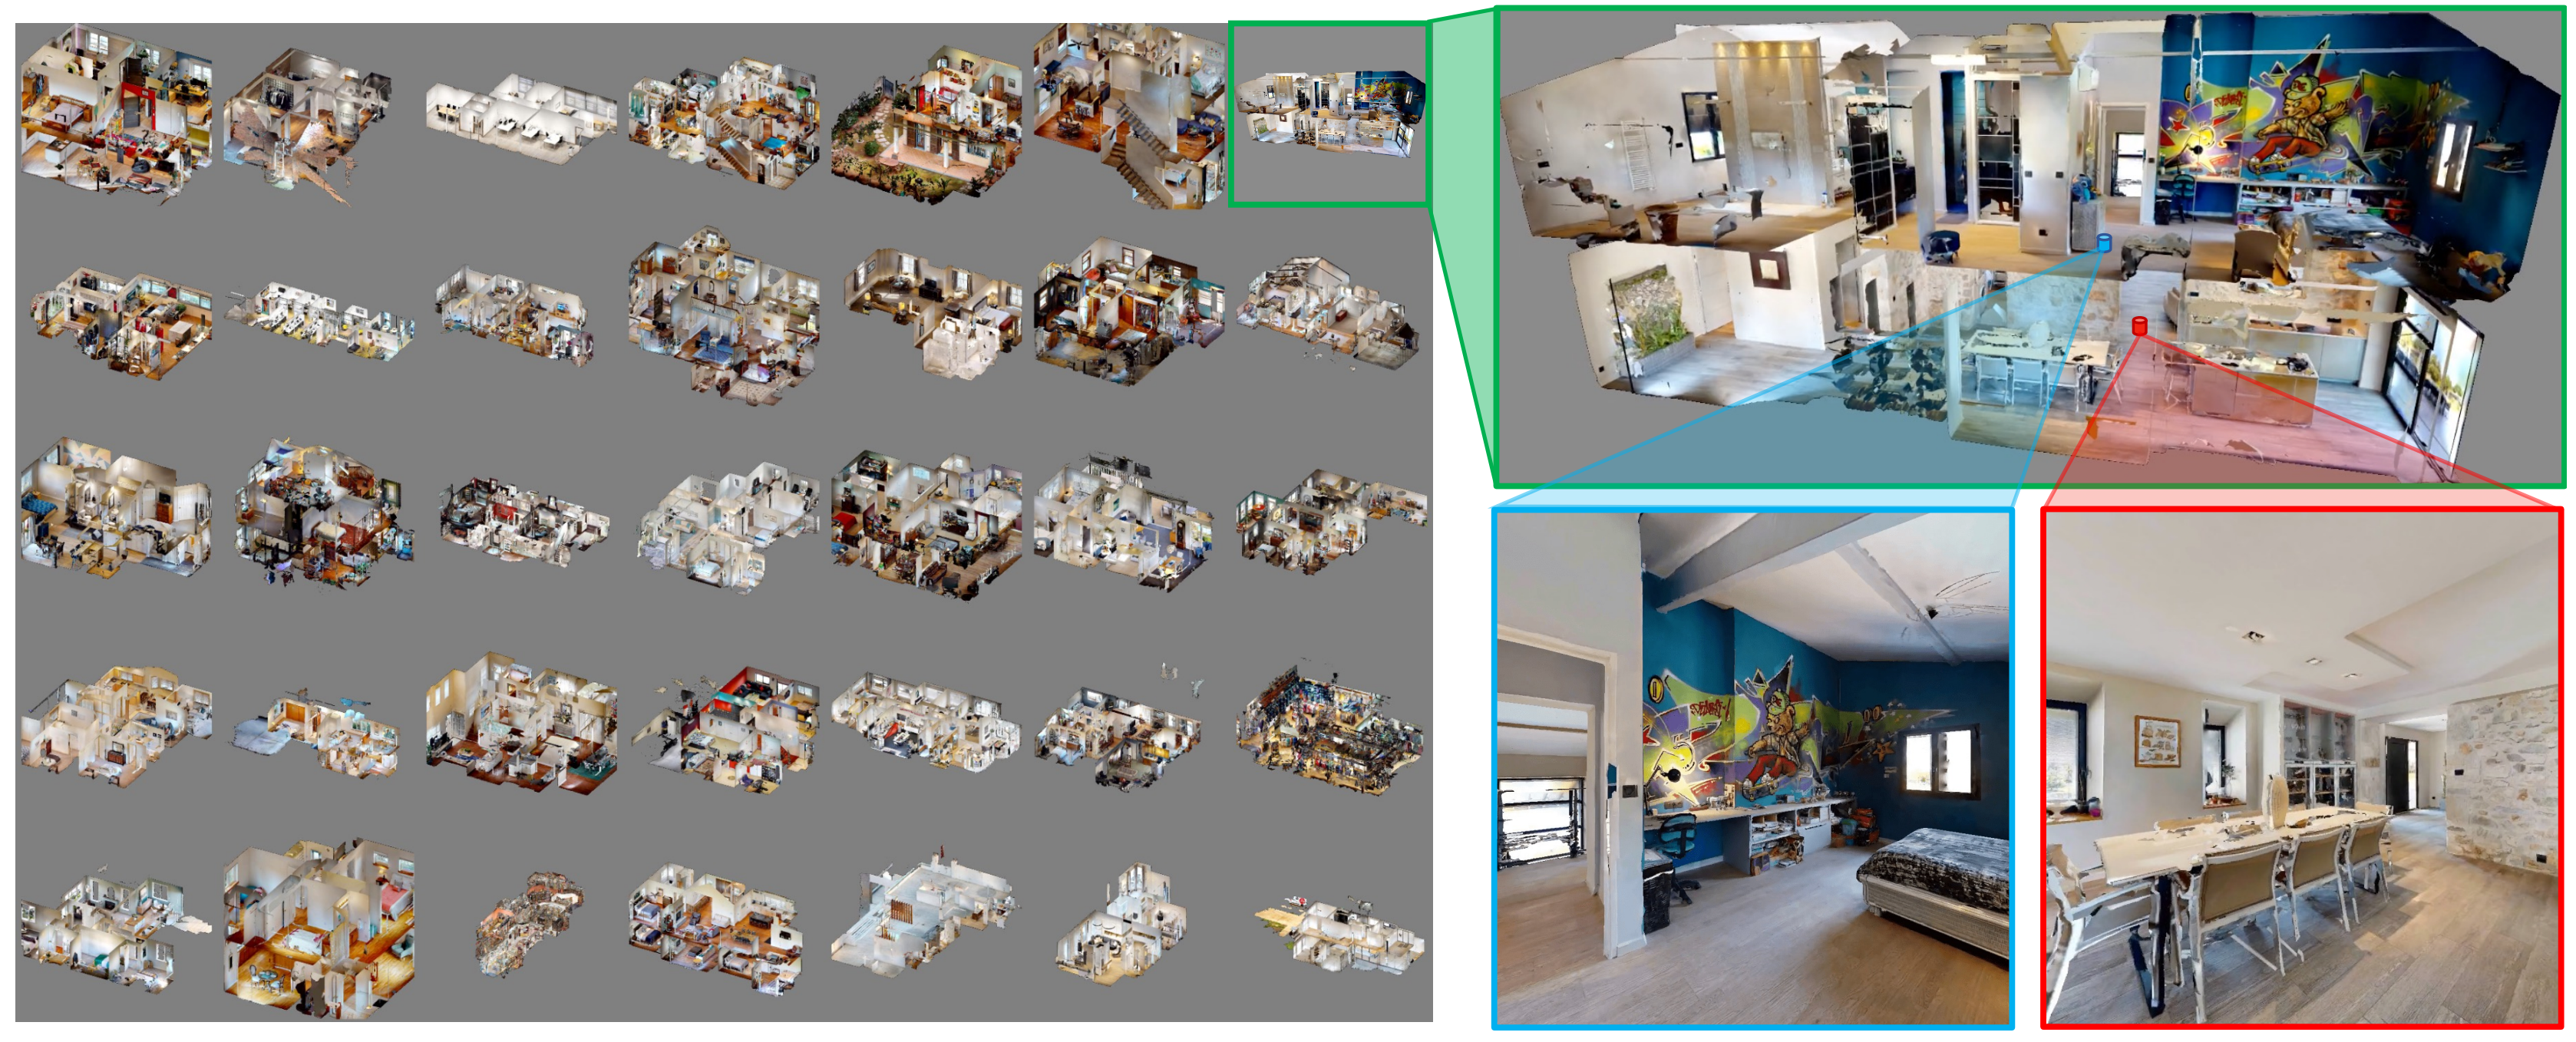
\includegraphics[width=1\linewidth]{Images/hm3d_images.png}
    \caption{This figure \cite{ramakrishnan2021habitat} shows various scenes from the HM3D dataset which we use for our testing. The left image shows a subset of the HM3D dataset and the top right image shows a close-up of one particular scene. The two images in the bottom right show snapshots from inside that scene}
    \label{fig:hm3d_imgs}
\end{figure}


\subsection{Spot URDF and Specifications}
We utilize the Boston Dynamics Spot robot URDF model for our experiments (see \textit{Figure} \ref{fig:SpotFig}). URDF stands for Unified Robot Description Format, and is a YAML document that defines the robot's physical structure, including links (analogous to bones), joints (which can be controlled like motors or muscles), and other data like appearance, collision meshes, and inertial data.

Boston Dynamics Spot robot URDF model contains 22 links and 17 joints, corresponding to the body, four articulated legs (each with hip–hip–knee actuation), sensor mounts, and auxiliary structural elements. In addition to these, defined outside of the URDF file in the task YAML file, we also create one depth sensor that's mounted in front of the robot and aligned with the robot's forward direction. This sensor provides dense per-pixel depth observations at each simulation step, enabling the robot to perceive information about its environment while excluding RGB or semantic data.

\subsection{Training Hyperparameters}
In training our reinforcement learning model, we use the following hyperparameters, defined in \texttt{ddpo\_pointnav\_quadruped.yaml}. See \textit{Listing \ref{fig:yml_hyperparameters}} for more details on this configuration.
\begin{lstlisting}[style=yamlstyle, caption={This YAML configuration specifies the reward structure and PPO training parameters for our PointNav policy.}, label={fig:yml_hyperparameters}]
RL:
  SUCCESS_REWARD: 10.0
  SLACK_REWARD: -0.002
  COLLISION_PENALTY: 0.003
  BACKWARDS_PENALTY: 0.003
  FULL_GEODESIC_DECAY: -1.0

  POLICY:
    name: "PointNavResNetPolicy"
    action_distribution_type: "gaussian"

  PPO:
    clip_param: 0.2
    ppo_epoch: 2
    num_mini_batch: 2
    value_loss_coef: 0.5
    entropy_coef: 0.01
    lr: 2.5e-4
    eps: 1e-5
    max_grad_norm: 0.2
    num_steps: 128
    use_gae: True
    gamma: 0.99
    tau: 0.95
    use_linear_clip_decay: False
    use_linear_lr_decay: False
    reward_window_size: 50
    hidden_size: 512
\end{lstlisting}

This YAML configuration specifies the reward structure and PPO training parameters for our PointNav policy. The most influential settings include the reward coefficients (SUCCESS\_REWARD, SLACK\_REWARD, COLLISION\_PENALTY, and BACKWARDS\_PENALTY) which define the agent's behavioral incentives. The FULL\_GEODESIC\_DECAY parameter controls whether distance-based reward shaping decays over an episode. Under the POLICY section, the network architecture (PointNavResNetPolicy) and action distribution type are defined. The PPO block contains optimization-critical parameters such as the clipping factor (clip\_param), learning rate (lr), number of rollout steps (num\_steps), discount factor (gamma), GAE parameters (use\_gae, tau), and architectural size (hidden\_size). Together, these values determine both the stability and performance of the RL training process in the environment.

\section{Results}
In this section, we present the performance of the trained navigation policy and evaluate how effectively the Spot robot learns to navigate within Habitat-Lab. We first analyze training metrics such as success rate and collision frequency to understand how the policy improves over time. We then examine qualitative evaluation rollouts, which illustrate how the agent uses depth perception to move through novel environments and how its behavior compares to the shortest-path solution. Together, these results provide both quantitative and qualitative evidence of the policy’s strengths and limitations.

\subsection{Training Results}
During training, we monitored multiple metrics to track the policy’s performance over time, including success rate, loss, reward, average collisions, etc. Of these metrics, we focus on episode success rate, and the average number of collisions per timestep across all parallel workers. These metrics provide complementary perspectives on how well the agent is learning the PointNav task and how its behavior evolves as training progresses.

\textit{Figure \ref{fig:success_plt}} shows the evolution of the success rate throughout the full training run. The raw per-episode values (green) exhibit substantial variability, which is expected given the diversity of scenes in the HM3D dataset and the stochastic nature of PPO rollouts. The smoothed curve (blue) reveals a clear trend: the policy rapidly improves during the first few million steps, reaching a peak success rate of approximately 80.38\% at around 6 million environment steps (after about 4.3 hours of training). This sharp rise indicates that the agent was able to quickly learn fundamental navigation behaviors such as orienting toward the goal, avoiding large obstacles, and maintaining forward motion.

After reaching its peak, the success rate begins to fluctuate and gradually declines over longer training horizons. This late-stage instability is a common characteristic of PPO and other methods, which continually update the policy using fresh samples that may differ significantly from earlier successful behaviors. As exploration continues and the distribution of visited states shifts, the policy may occasionally overfit to short-term behaviors or experience degradation due to high-variance updates. For our model evaluation (see \textit{Section \ref{sec:eval_results}}), we use the training checkpoint that was created closest to this peak in the success rate near 6 million steps.

A similar pattern appears in the collision metric shown in \textit{Figure \ref{fig:collisions_plt}}. Collisions decrease substantially during the early stages of learning, dropping from initial high values to a local minimum at roughly the same point where success rate peaks. This strong correlation suggests that improved obstacle avoidance directly contributes to higher navigation success. After this minimum, the average collision count stabilizes and slowly increases, mirroring the long-term decline in success rate. This indicates that the agent becomes slightly less conservative in its motion as training progresses, which can help exploration but may also lead to more collisions in cluttered environments.

These results show that the Spot agent is capable of learning meaningful and effective navigation strategies using only depth perception and goal direction information. The early phases of training produce strong gains in both success rate and collision avoidance, demonstrating that the PPO-based policy can acquire stable locomotion and obstacle-aware behavior within the \texttt{kin2dyn} framework. The later-stage fluctuations highlight some of the inherent challenges of long-term on-policy training, suggesting that techniques such as curriculum learning, reward adjustment, or periodic policy snapshotting could further stabilize performance in future work.

\begin{figure}
    \centering
    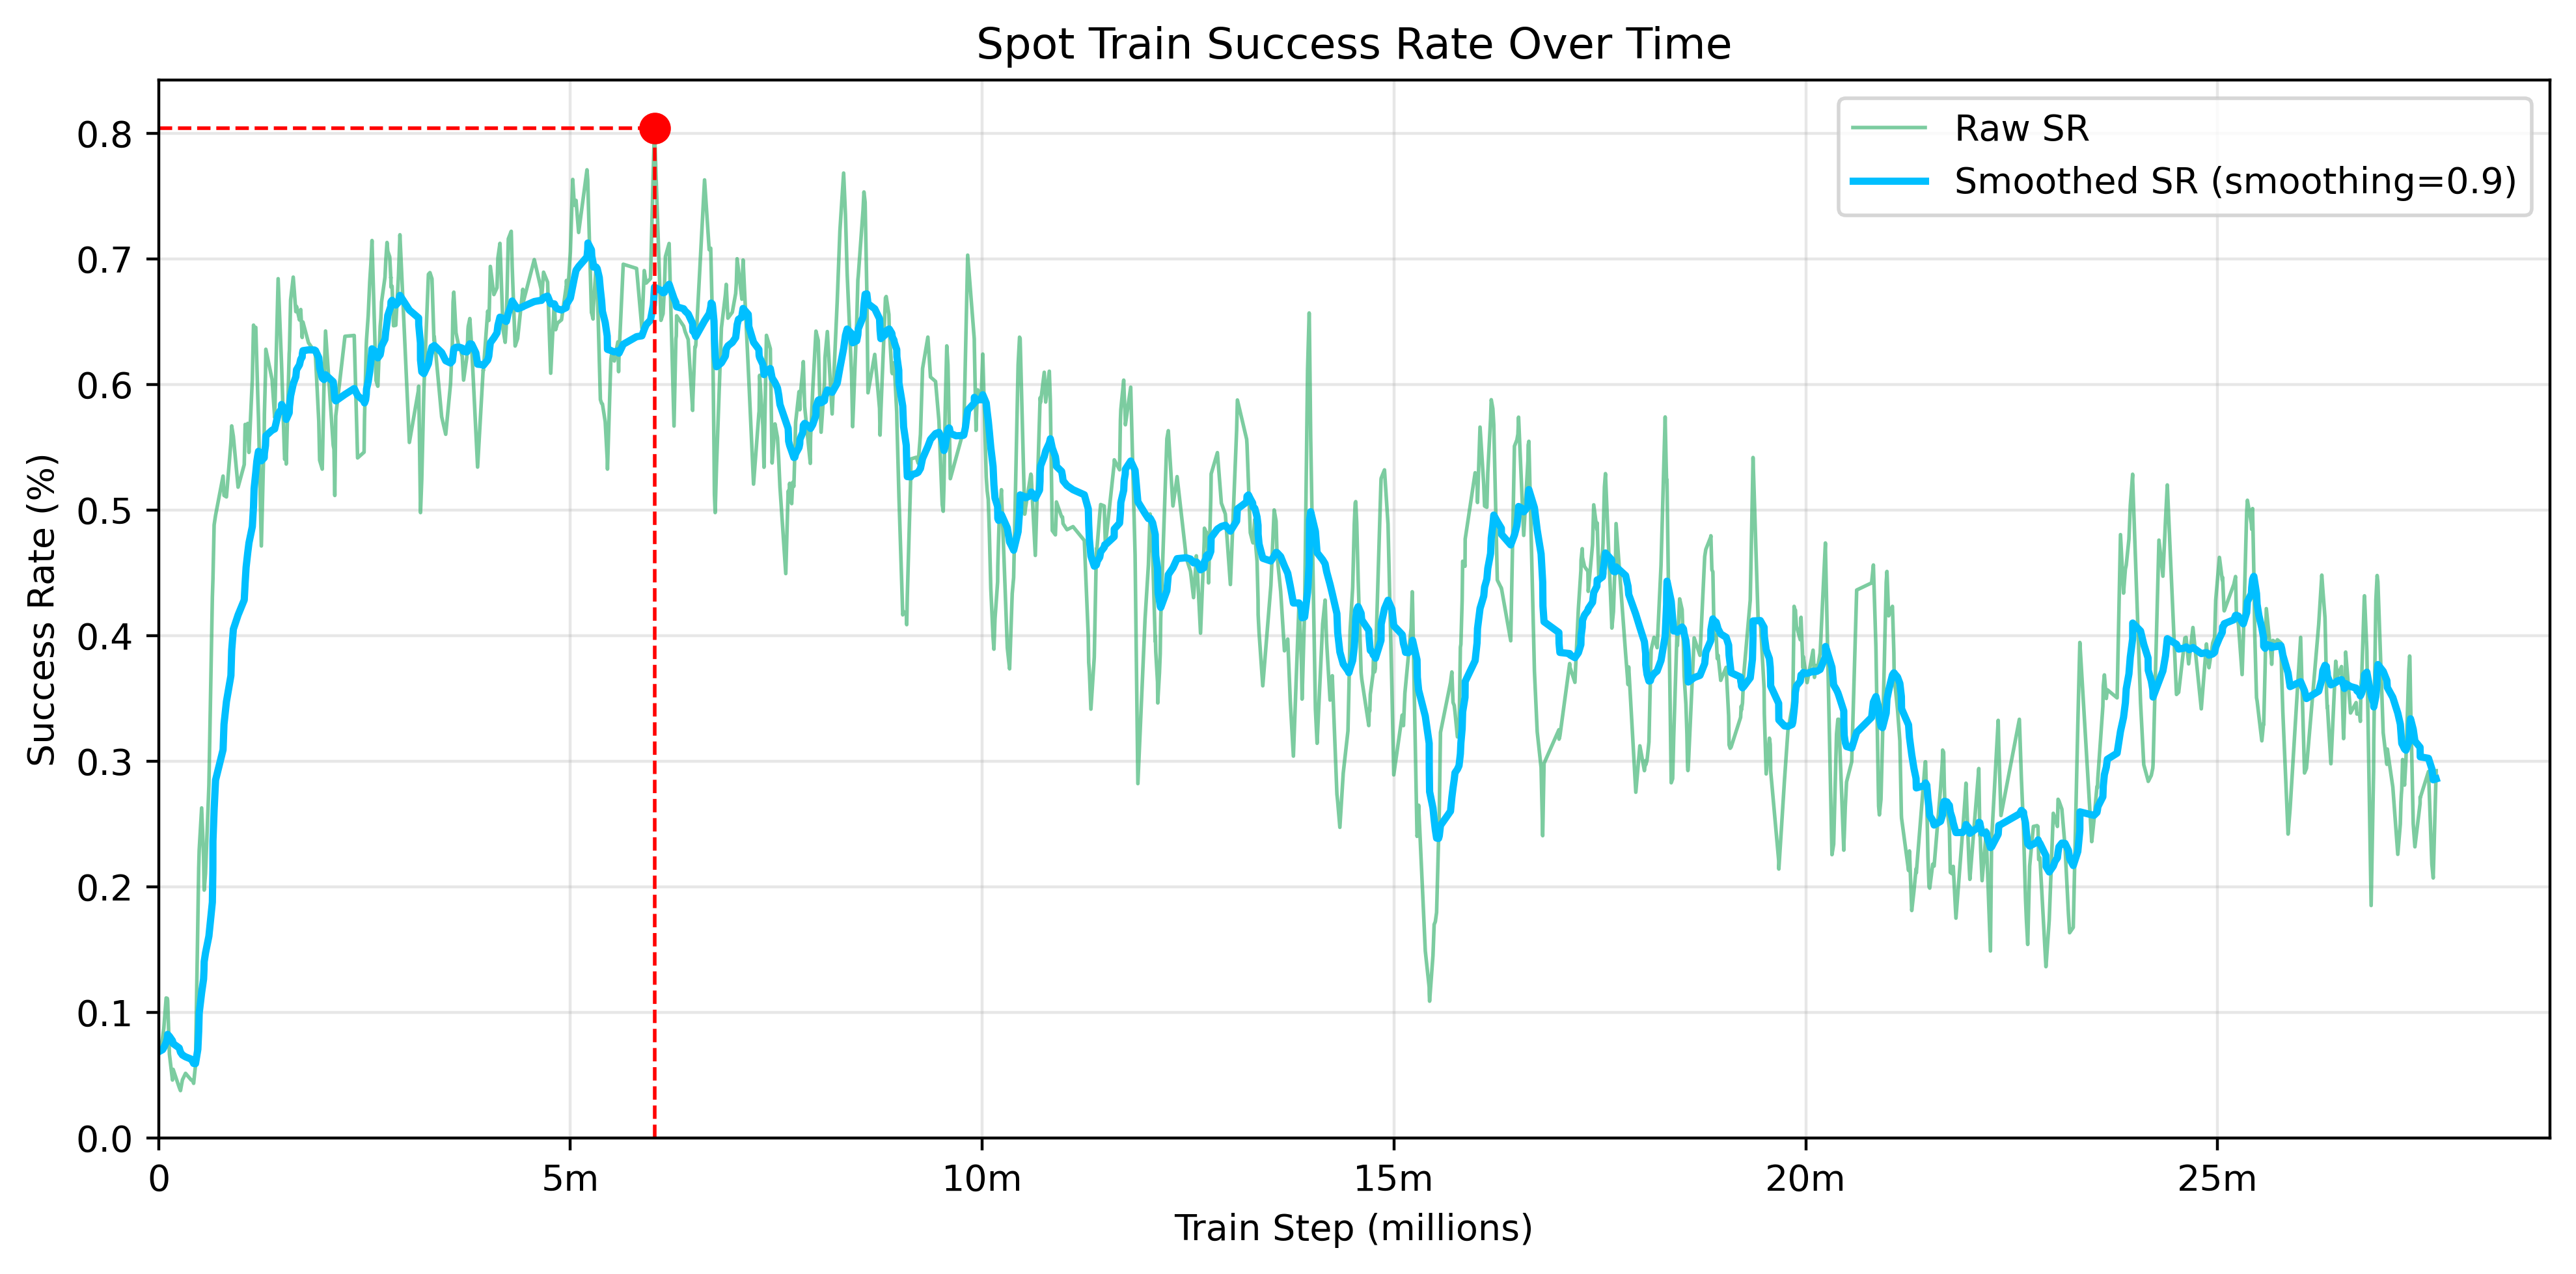
\includegraphics[width=\linewidth]{Images/spot_success.png}
    \caption{This chart displays the training success rate of the Spot robot over time. The green trace shows the raw per-episode success rate, while the blue trace shows an exponentially smoothed version (smoothing = $0.9$). The red marked point denotes the maximum observed success rate ($80.38\%$) and its corresponding training step ($\sim6.02$ million steps). This point was reached after about 4.3 hours of training. The plot shows early rapid improvement followed by long-term fluctuations and gradual decline as training progresses.}
    \label{fig:success_plt}
\end{figure}

\begin{figure}
    \centering
    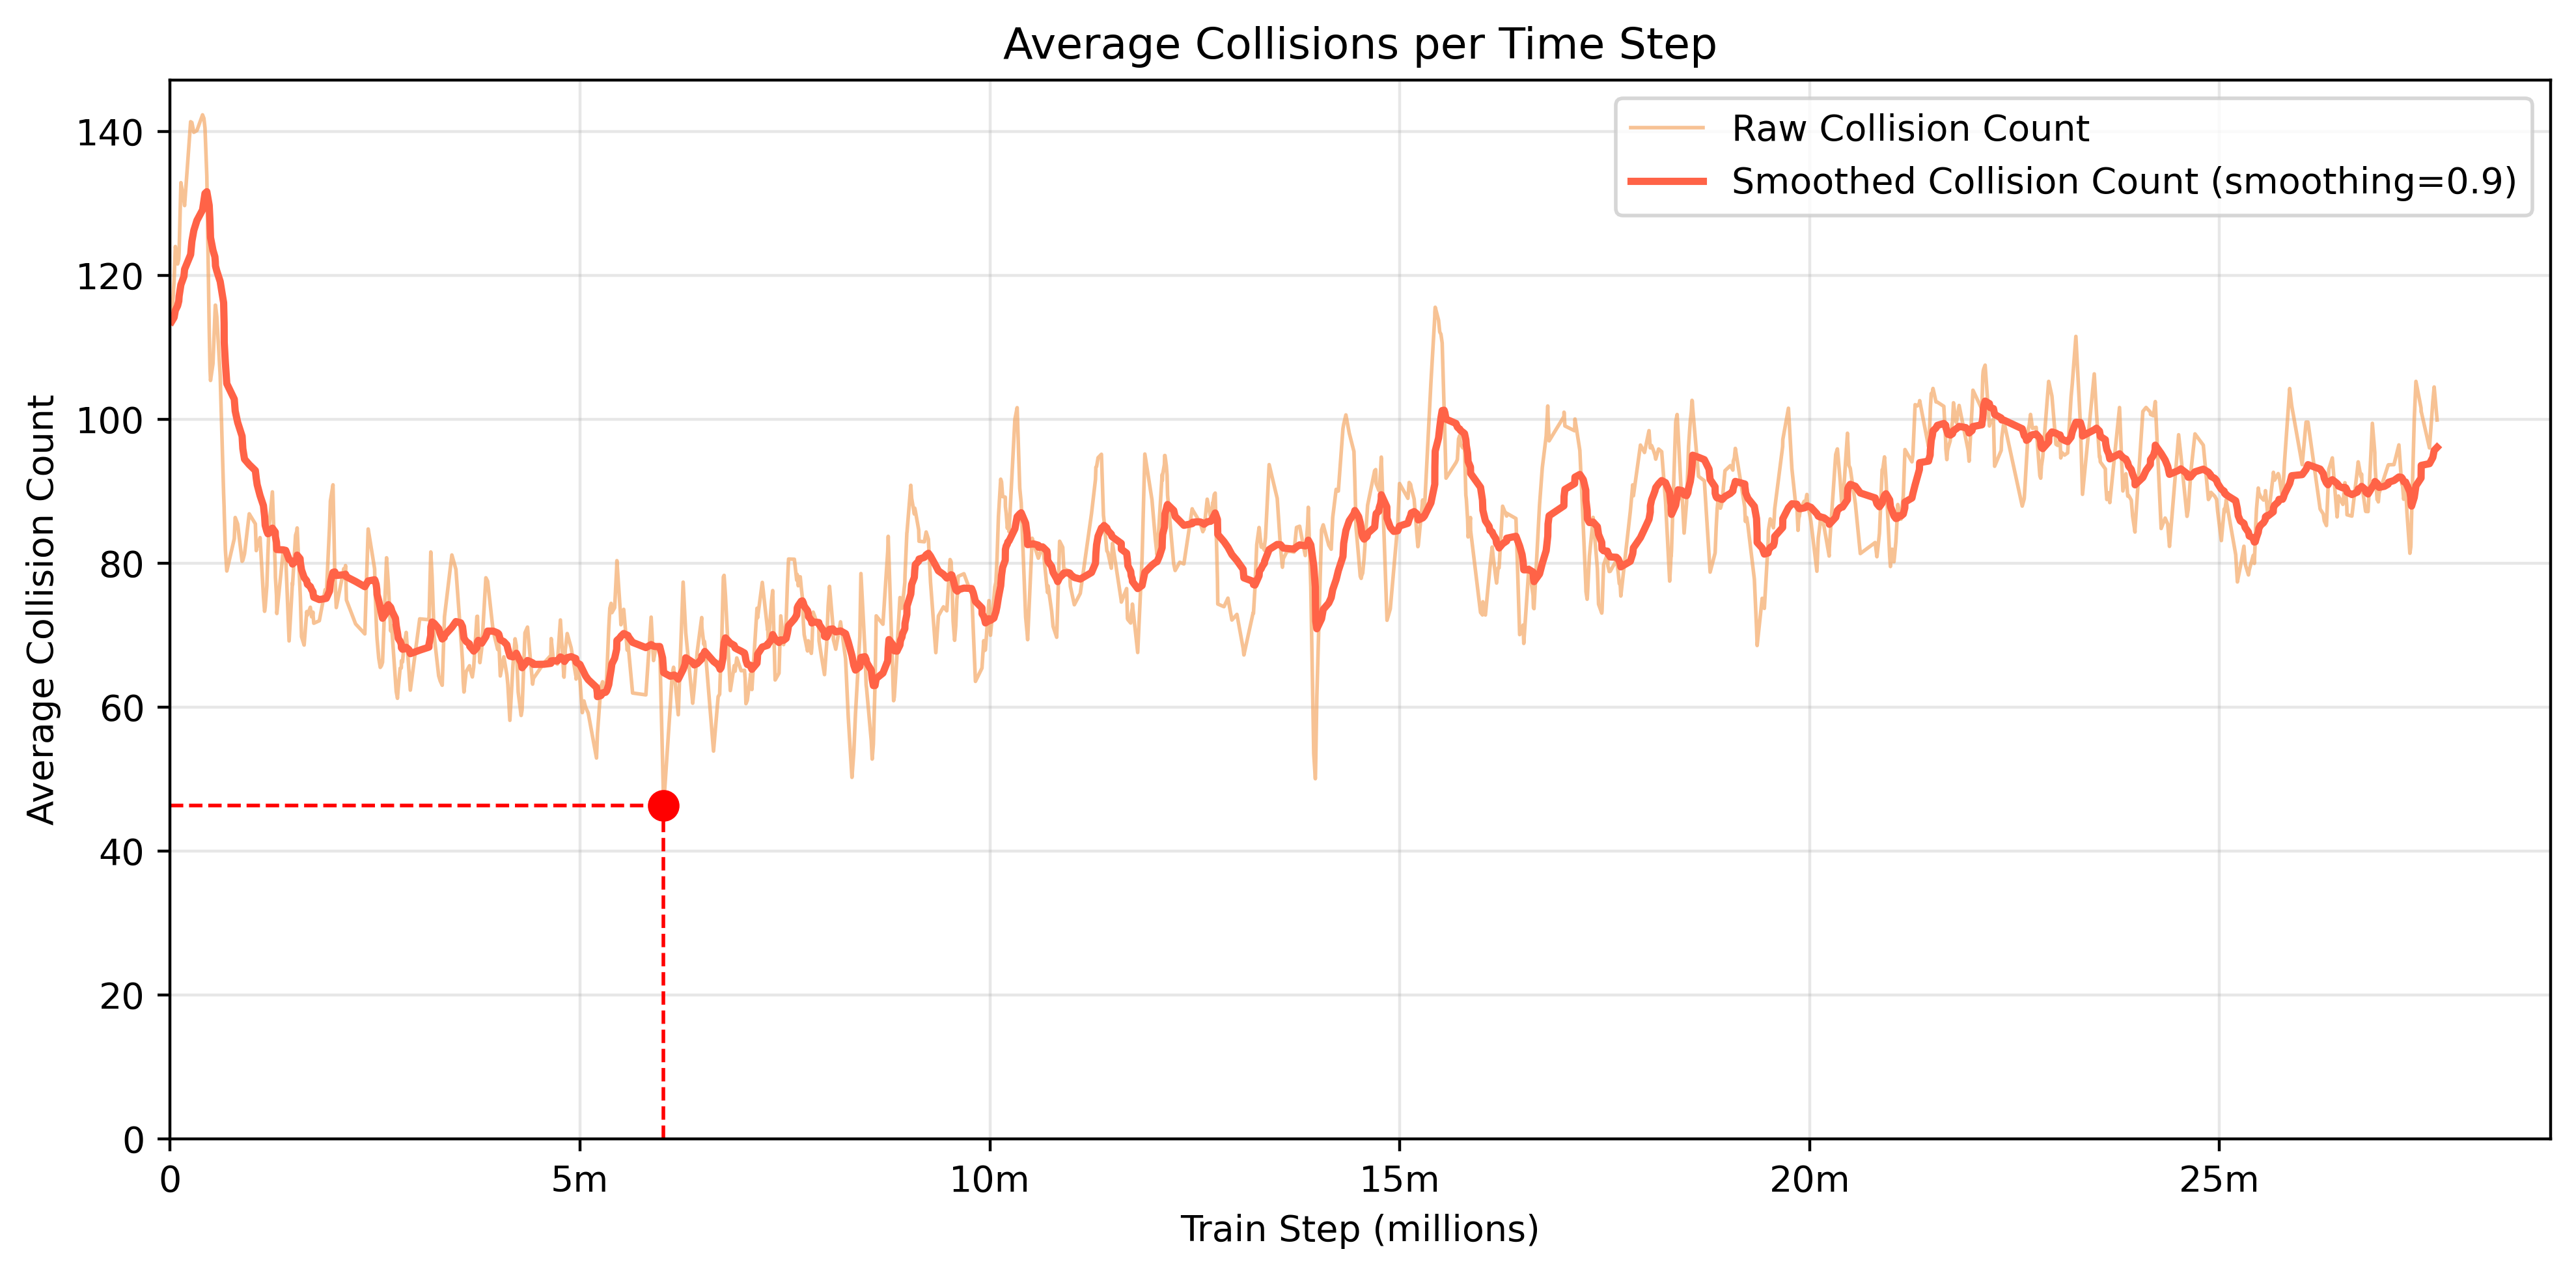
\includegraphics[width=1\linewidth]{Images/spot_collisions.png}
    \caption{This graph shows the average number of collisions during each time step of the simulation. Collisions are counted as contact between any part of the robot with part of the environment's mesh. This is calculated by averaging the number of collision across all of the parallel worker environments (in our case 8).}
    \label{fig:collisions_plt}
\end{figure}


\subsection{Evaluation Results} \label{sec:eval_results}
To better understand the behavior of the trained policy during navigation, we generated evaluation rollouts and visualized the agent’s motion inside the simulated environment. \textit{Figure \ref{fig:video_frame}} shows a representative frame from one of these evaluation videos. The visualization provides three complementary perspectives on the agent’s behavior.

The left panel shows a third-person view of the simulated Spot robot as it moves through the environment. This view highlights the robot’s high-level locomotion decisions, such as turning behavior, obstacle avoidance, and overall path direction. The center panel displays the depth image captured by the robot’s onboard depth sensor at that exact moment. This depth map is the primary source of visual information used by the policy, allowing the agent to detect obstacles, walls, and open space directly in front of it. The right panel offers a top-down visualization of the environment. Free space is shown in dark gray, obstacles in white, and the area the agent has already observed in light gray. The blue trajectory represents the robot’s executed path during evaluation, while the green path shows the shortest path to the target that's pre-computed for that particular scene. Comparing these two paths gives insight into how closely the learned policy follows the most efficient route and how it adapts when navigating around unseen obstacles or complex environmental geometry. A robot trained with a perfect model should always be able to follow the green line exactly without deviations, regardless of the obstacles or layout of the environment, although obtaining a perfect model is in practice impossible.

This visualization helps to illustrate how the robot integrates depth perception with its learned navigation policy to move through unseen indoor environments. It provides a clear, qualitative understanding of the robot’s decision-making process during evaluation, complementing the quantitative metrics reported in the following sections.

\begin{figure}
    \centering
    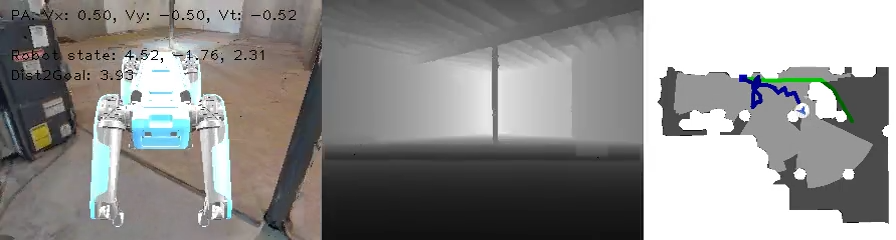
\includegraphics[width=1\linewidth]{Images/Screenshot from episode=9-ckpt=0-distance_to_goal=0.23-episode_distance=8.40-success=1.00-spl=0.56-collisions.count=20.00.mp4 - 1.png}
    \caption{This figure is a frame from a generated evaluation video after training. The left panel shows the simulated robot inside the environment from the third person. The center panel shows what the the robot is ``seeing" from it's onboard depth sensor. The right panel depicts the empty space in the environment (dark gray), the agent's observed space (light gray), obstacles (white), the agent (the arrow), the agent's path (the blue line), and the calculated shortest path in this specific scene (green). }
    \label{fig:video_frame}
\end{figure}

\section{Real-World Transfer}
Although this project focuses on training and evaluating navigation behaviors inside the Habitat-Lab simulation environment, the methods developed here have clear potential for deployment on a real Boston Dynamics Spot robot, or other robotic systems in the real-world. The \texttt{kin2dyn} framework already mirrors Spot’s kinematics and uses a velocity-based control interface similar to the real API, making the learned policy structurally compatible with the mirrored hardware components. With additional system integration, the navigation policy trained in Habitat could easily be transferred to real-world environments.

A next step would be bridging the gap between Habitat’s idealized sensors and Spot’s actual depth and perception hardware. This typically involves adding noise models, adjusting the depth range, and incorporating domain randomization to make the policy more robust to lighting, reflections, and real-world surface properties. The GPS+Compass goal sensor used in Habitat would also need to be replaced with a real localization method, such as Spot’s onboard visual-inertial SLAM or an external tracking system. Once these components are aligned, the velocity commands produced by the learned policy could be executed directly by Spot’s API.

Transferring this policy to a physical robot opens up several meaningful applications. Indoors, Spot could autonomously navigate warehouses, laboratories, or construction sites to inspect equipment or collect sensor readings. In search-and-rescue settings, a depth-based navigation policy would allow Spot to move through cluttered or partially collapsed structures without relying on fragile visual features. In research environments, the system could serve as a foundation for higher-level tasks such as autonomous mapping, patrolling, or multi-robot coordination.

\section{Conclusion}
In this project, we demonstrated that reinforcement learning methods can be used to train a quadrupedal robot—specifically the Boston Dynamics Spot—to perform point-to-point indoor navigation using only depth observations and goal direction information. By leveraging Habitat-Lab, the \texttt{kin2dyn} extension, and PPO-based training with distributed rollout collection, we were able to efficiently generate large amounts of diverse experience in photorealistic 3D scenes. Our experiments show that the learned policy develops meaningful navigation behaviors, including obstacle avoidance, goal-directed motion, and stable locomotion within cluttered indoor environments.

The results provide evidence that high-fidelity simulation can serve as an effective platform for developing legged navigation policies without requiring physical hardware during training. While performance fluctuates during long-term on-policy optimization, the agent consistently reaches strong intermediate performance, achieving high success rates and reduced collisions across challenging HM3D environments. These behaviors were further validated through qualitative evaluation rollouts, which illustrate how the policy interprets depth input and navigates through unseen spaces.

Overall, this work highlights the practicality and value of simulation-driven RL for legged robotics. The methods explored here form a foundation for future deployment on real hardware, where additional techniques such as sensor modeling, domain randomization, and improved localization will help close the sim-to-real gap. As legged robots continue to be adopted across research, industry, and safety-critical applications, scalable simulation-based training pipelines like the one developed in this project will be essential for building robust, autonomous navigation capabilities.

\subsection{Key Takaways}
Working on this project taught me a lot about both reinforcement learning and the practical challenges of training a legged robot in simulation. One of the biggest things I learned is how much small design choices matter—changing a reward coefficient, adjusting an action range, or tweaking the observation setup could noticeably change the robot’s behavior. PPO also turned out to be a bit unpredictable: it learns good behaviors fairly quickly, but if you keep training for too long, performance can drift or even get worse. Because of that, saving checkpoints and watching the metrics closely ended up being more important than I originally expected.

I also got a much better understanding of how Habitat-Lab and the \texttt{kin2dyn} framework work together. Using velocity commands instead of low-level joint control made the whole problem far more manageable and let the policy focus on navigation instead of raw locomotion. Running multiple environments in parallel wasn’t just a speed improvement—it really helped the agent see more diverse scenes early on, which seemed to make learning more stable.

Finally, this project made it very clear that there’s still a gap between simulation and the real world. Even though the policy works well in Habitat, transferring it to an actual Spot would require handling noise, sensor differences, and other details that simulation smooths out. But overall, I came away with a stronger appreciation for how powerful simulation can be for robotics research, and how much it can accelerate progress before ever touching real hardware.

\newpage
\printbibliography
\end{document}
